\documentclass[a4paper, 10pt, oneside]{report}
\usepackage[utf8]{inputenc}
 

% ==============================================================
% File     : lib/includes.tex
% Date     : 26 Nov. 2021
% Revision : 30 July 2022
% Creator  : Marco Peressutti
% ==============================================================

% ==============================================================
% $package-name$ : type     : $description$
% --------------------------------------------------------------
% amsmath        : math     : AMS mathematical facilities for LaTeX
% amssymb        : math     : AMS symbols
% amsthm         : math     : Typesetting theorems (AMS style)

% babel          : biblio   : Multilingual suppor for latex ...
% biblatex       : biblio   : Sophisticated Bibliographies in LaTeX
% bm             : math     : Access bold symbols in maths mode
% booktabs       : tables   : Publication quality tables in LaTeX

% cancel         : math     : Place lines through maths formulae
% csquotes       : misc     : Context sensitive quotation facilities

% dirtytalk      : misc     : A package to typeset quotations easier

% empheq         : math     : EMPHasizing EQuations
% enumitem       : misc     : Control layout of itemize, enumerate, description

% fancyhdr       : page     : Extensive control of page headers and footers in LaTeX2epsilon
% fontenc        : font     : Standard package for selecting font encodings

% geometry       : page     : Flexible and complete interface to document dimensions
% glossaries     : misc     : Create glossaries and lists of acronym
% graphicx       : graphics : Enhanced suppoort for graphics

% hyperref       : misc     : Extensive support for hypertext in LaTeX

% listings       : code     : Typeset source code listings using LaTeX
% lmodern        : font     : Latin modern fonts in outline formats

% makecell       : misc     : Tabular column heads and multilined cell
% marginnote     : page     : Notes in the margin, even where \marginpar fails
% mathtools      : math     : Mathematical tools to use with amsmath
% microtype      : font     : Subliminal refinements towards typographical perfection
% minitoc        : misc     : Produce a table of contents for each chapter, part or section

% nicematrix     : math     : Improve the typesetting of mathematical matrices with PGF

% pifont         : font     : Access to PostScript standard Symbol and Dingbats fonts

% setspace       : misc     : Set space between lines
% subcaption     : graphics : Support for sub-captions

% tabularx       : tables   : Tabulars with adjustable-width columns
% todonotes      : page     : Marking things to do in a LaTeX document

% xcolor         : misc     : Driver-independent color extensions for LaTeX and pdfLaTeX
% xfrac          : math     : Split-level fractions in LaTeX2epsilon
% ==============================================================

\usepackage[right=30.2mm, left=28.4mm, marginparwidth=75pt, top=20mm]{geometry}
%\usepackage[a4paper, marginparwidth=75pt, total={10cm, 10cm}]{geometry}

\usepackage[english]{babel} 
\usepackage[bibstyle=numeric, backend=biber, sorting=nty]{biblatex}

\usepackage{listings}

\usepackage[T1]{fontenc}    
\usepackage{lmodern}        
\usepackage{microtype}      
\usepackage{pifont}

\usepackage{graphicx}       
\usepackage{subcaption}

\usepackage{amsmath} 
\usepackage{amssymb} 
\usepackage{mathtools} 
\usepackage{amsthm}
\usepackage[makeroom]{cancel}
\usepackage{empheq}
\usepackage{nicematrix}
\usepackage{xfrac}
\usepackage{bm}

\usepackage{tabularx}
\usepackage{booktabs}
%\usepackage{minitoc}

\usepackage{marginnote}
\usepackage{todonotes}
\usepackage{fancyhdr}

\usepackage{dirtytalk}      
\usepackage{csquotes}
\usepackage[acronym, nonumberlist, seeautonumberlist]{glossaries}
\usepackage{hyperref}
\usepackage{setspace}
\usepackage{enumitem}
\usepackage{xcolor}
\usepackage{makecell}

\usepackage[most,many,breakable]{tcolorbox}

\usepackage{titlesec, titletoc} %// TODO: add these to the description above
\usepackage{algorithm, algorithmic}
% ==============================================================
% File     : lib/acronyms.tex
% Date     : 30 July 2022
% Revision : 30 July 2022
% Creator  : Marco Peressutti
% ==============================================================

\newacronym{HW}{HW}{Hardware}
\newacronym{SW}{SW}{Software}
\newacronym{OS}{OS}{Operating System}
\newacronym{RTOS}{RTOS}{Real-Time Operating System}
\newacronym{RM}{RM}{Rate Monotonic}
\newacronym{DM}{DM}{Deadline Monotonic}
\newacronym{EDF}{EDF}{Earliest Deadline First}
\newacronym{IPC}{IPC}{Inter-Process Communication}
\newacronym{I/O}{I/O}{Input/Ouput}
% ==============================================================
% File     : lib/commands.tex
% Date     : 26 Nov. 2021
% Revision : 30 July 2022
% Creator  : Marco Peressutti
% ==============================================================

\defbibheading{bibempty}{}
% ==============================================================
% NEW-COMMANDS:
% ==============================================================

% \M         : matrix with square    delimiters/brackets
% \B         : matrix with curly     delimiters/brackets
% \und       : underline math expression in math mode
% \pd        : (first  order) partial derivative
% \td        : (first  order) total   derivative
% \pdd       : (second order) partial derivative 
% \tdd       : (second order) total   derivative
% \omissis   : three dots surrounded by square brackets
% \pexp      : pre exponent (#1) of symbol (#2) where \pexp{#1}{#2} 
% \ret       : left arrow symbol as exponent 
% \smalltodo : [internal] DO NOT USE 
% \side      : size notes (yellow line to the side of the page with text)
% \pside     : phantom side (used in environment where the \side causes compilation errors)
% \ceil      : ceil  brackets
% \floor     : floor brackets 
% \degr      : degree symbol (just an exponent with circle in front of the number)

\newcommand{\M}[1]{\begin{bmatrix}#1\end{bmatrix}}
\newcommand{\und}[1]{\underline{#1}}
\newcommand{\B}[1]{\begin{Bmatrix}#1\end{Bmatrix}}
\newcommand{\pd}[2]{\cfrac{\partial#1}{\partial#2}}
\newcommand{\td}[2]{\cfrac{d#1}{d#2}}
\newcommand{\pdd}[2]{\cfrac{\partial^2#1}{\partial#2^2}}
\newcommand{\tdd}[2]{\cfrac{d^2#1}{d#2^2}}
\newcommand{\omissis}{[\textellipsis\unkern]}
\newcommand{\pexp}[2]{\prescript{#1}{}{#2}{}{}}
\newcommand{\ret}[1]{{#1}^{\leftarrow}}
\newcommand{\smalltodo}[2][]{\todo[caption={#2}, #1, backgroundcolor=white!20!white, bordercolor=white]{\begin{spacing}{0.5}\texttt{#2}\end{spacing}}}
\newcommand{\side}[1]{\smalltodo[size=\footnotesize]{#1}\textbf{#1}}
\newcommand{\pside}[1]{\smalltodo[size=\footnotesize]{#1}}
\newcommand{\ceil}[1]{\left\lceil #1 \right\rceil}
\newcommand{\floor}[1]{\left\lfloor #1 \right\rfloor}
\newcommand{\degr}[1]{^{\circ\!#1}}

% ==============================================================
% RE-NEW-COMMANDS:
% ==============================================================

% prettier \theta symbol
\renewcommand{\theta}{\vartheta}
% prettier \epsilon symbol
\renewcommand{\epsilon}{\varepsilon}
% I have no clue what \arraystretch does prolly used internally in itemize/enumerate environment
\renewcommand{\arraystretch}{1.3}

% ==============================================================
% DECLARES:
% ==============================================================

% \abs      : absolute value operator/delimiters (i.e. |  expression  |)
% \norma    : norm           operator/delimiters (i.e. || expression ||)
% \minimize : "minimize" that allows to write things just under the symbol 
% \argmin   : "argmin" that allows to write things just under the symbol
\DeclarePairedDelimiter\abs{\lvert}{\rvert}
\DeclarePairedDelimiter{\norma}{\lVert}{\rVert}
\DeclareMathOperator*{\minimize}{minimize}
\DeclareMathOperator*{\argmin}{argmin}


% ==============================================================
% MISC:
% ==============================================================

% more compact representtation of itemize
\setitemize{noitemsep,topsep=10pt,parsep=0pt,partopsep=0pt}

% colors
\definecolor{codegreen}{rgb}{0,0.6,0}
\definecolor{codegray}{rgb}{0.5,0.5,0.5}
\definecolor{codepurple}{rgb}{0.58,0,0.82}
\definecolor{backcolour}{rgb}{0.95,0.95,0.92}
\definecolor{myb}{RGB}{45, 111, 177}
\definecolor{myr}{RGB}{199, 68, 64}
\definecolor{myg}{RGB}{90, 199, 90}

% Code snippets style
\lstdefinestyle{mystyle}{
    backgroundcolor=\color{backcolour},   
    commentstyle=\color{codegreen},
    keywordstyle=\color{magenta},
    numberstyle=\tiny\color{codegray},
    stringstyle=\color{codepurple},
    basicstyle=\ttfamily\footnotesize,
    breakatwhitespace=false,         
    breaklines=true,                 
    captionpos=b,                    
    keepspaces=true,                 
    numbers=left,                    
    numbersep=5pt,                  
    showspaces=false,                
    showstringspaces=false,
    showtabs=false,                  
    tabsize=2
}
\lstset{style=mystyle}

\makeatletter
\newcommand\incircbin
{%
  \mathpalette\@incircbin
}
\newcommand\@incircbin[2]
{%
  \mathbin%
  {%
    \ooalign{\hidewidth$#1#2$\hidewidth\crcr$#1\bigcirc$}%
  }%
}
\newcommand{\ooplus}{\incircbin{+}}     % A circle with a plus  inside
\newcommand{\oominus}{\incircbin{-}}    % A circle with a minus inside
\newcommand{\oocirca}{\incircbin{\sim}} % A circle with a tilde inside
\makeatother

\newcommand{\cmark}{\ding{51}} % literally a  tick
\newcommand{\xmark}{\ding{55}} % literally an X

% equal with symbol on top
\newcommand\equal[1]{\stackrel{\mathclap{\footnotesize\mbox{#1}}}{=}}

% text without double lined line
\newcommand{\textbetweendoublerules}[2][.4pt]{%
  \par\addvspace{\topsep}
  \noindent\makebox[\textwidth]{%
    \sbox0{\quad#2\quad}%
    \dimen0=.5\dimexpr\ht0+#1\relax
    \dimen2=-.5\dimexpr\ht0-#1\relax
    \dimen4=.5\dimexpr\textwidth-\wd0\relax
    \setbox2=\vbox to \ht0{%
      \vss
      \hrule width \dimen4 height #1
      \kern 4\dimexpr#1\relax
      \hrule width \dimen4 height #1
      \vss
    }%
    \copy2 \box0 \box2
  }\par\nopagebreak\addvspace{\topsep}%
}


% red box used for examples
\makeatletter
\newtcbtheorem{iexample}{Example}{enhanced,
	breakable,
	colback=white,
	colframe=myr!80!black,
	attach boxed title to top left={yshift*=-\tcboxedtitleheight},
	fonttitle=\bfseries,
	title={#2},
	boxed title size=title,
	boxed title style={%
			sharp corners,
			rounded corners=northwest,
			colback=tcbcolframe,
			boxrule=0pt,
		},
	underlay boxed title={%
			\path[fill=tcbcolframe] (title.south west)--(title.south east)
			to[out=0, in=180] ([xshift=5mm]title.east)--
			(title.center-|frame.east)
			[rounded corners=\kvtcb@arc] |-
			(frame.north) -| cycle;
		},
	#1
}{def}
\makeatother

% blue box used for definitions
\makeatletter
\newtcbtheorem{idefinition}{Definition}{enhanced,
	breakable,
	colback=white,
	colframe=myb!80!black,
	attach boxed title to top left={yshift*=-\tcboxedtitleheight},
	fonttitle=\bfseries,
	title={#2},
	boxed title size=title,
	boxed title style={%
			sharp corners,
			rounded corners=northwest,
			colback=tcbcolframe,
			boxrule=0pt,
		},
	underlay boxed title={%
			\path[fill=tcbcolframe] (title.south west)--(title.south east)
			to[out=0, in=180] ([xshift=5mm]title.east)--
			(title.center-|frame.east)
			[rounded corners=\kvtcb@arc] |-
			(frame.north) -| cycle;
		},
	#1
}{def}
\makeatother

% green box used for theorems
\makeatletter
\newtcbtheorem{itheorem}{Theorem}{enhanced,
	breakable,
	colback=white,
	colframe=myg!80!black,
	attach boxed title to top left={yshift*=-\tcboxedtitleheight},
	fonttitle=\bfseries,
	title={#2},
	boxed title size=title,
	boxed title style={%
			sharp corners,
			rounded corners=northwest,
			colback=tcbcolframe,
			boxrule=0pt,
		},
	underlay boxed title={%
			\path[fill=tcbcolframe] (title.south west)--(title.south east)
			to[out=0, in=180] ([xshift=5mm]title.east)--
			(title.center-|frame.east)
			[rounded corners=\kvtcb@arc] |-
			(frame.north) -| cycle;
		},
	#1
}{def}
\makeatother


% green box used for theorems
\makeatletter
\newtcbtheorem{ilemma}{Lemma}{enhanced,
	breakable,
	colback=white,
	colframe=myg!80!black,
	attach boxed title to top left={yshift*=-\tcboxedtitleheight},
	fonttitle=\bfseries,
	title={#2},
	boxed title size=title,
	boxed title style={%
			sharp corners,
			rounded corners=northwest,
			colback=tcbcolframe,
			boxrule=0pt,
		},
	underlay boxed title={%
			\path[fill=tcbcolframe] (title.south west)--(title.south east)
			to[out=0, in=180] ([xshift=5mm]title.east)--
			(title.center-|frame.east)
			[rounded corners=\kvtcb@arc] |-
			(frame.north) -| cycle;
		},
	#1
}{def}
\makeatother


% command to use the definition box \definition{Name}{Verbose definition of Name}
\newcommand{\definition}[2]{\begin{idefinition}{#1}{}#2\end{idefinition}}
% command to use the definition box \definition{(optional) Example title}{Verbose description of Example}
\newcommand{\example}[2]{\begin{iexample}{#1}{}#2\end{iexample}}
% command to use the definition box \definition{(optional) Example title}{Verbose description of Example}
\newcommand{\theorem}[2]{\begin{itheorem}{#1}{}#2\end{itheorem}}
\newcommand{\lemma}[2]{\begin{ilemma}{#1}{}#2\end{ilemma}}

% used to make table of contents for each part
\titleclass{\part}{top}
\titleformat{\part}
  {\centering\normalfont\Huge\bfseries}{}{0pt}{}
\setcounter{secnumdepth}{5}

\title{145071 - Real time operating systems and middleware}
\author{Marco Peressutti\\230403\\marco.peressutti@studenti.unitn.it}
\date{\today}

\includeonly{
chapters/01-Introduction,
chapters/02-RTScheduling,
chapters/03-TimeDemandAnalysis,
chapters/04-SharedResources,
chapters/05-DynamicScheduling,
chapters/06-AperiodicServers,
chapters/07-EDFScheduling,
chapters/08-Kernel,
chapters/09-TimerandClock,
chapters/10-Nonpreemptablesection,
chapters/0A-MarkovChains}

\addbibresource{bib/bibliografia.bib}							% agguinge database bibliografico
\graphicspath{{images/}}	
\makeglossaries

\begin{document}
\maketitle
\tableofcontents

\chapter{Introduction to the course}
\section{Overview of the course}

\begin{itemize}
\item \side{\textbf{Real time systems}}

About the topic we will cover:
\begin{itemize}
\item \side{Real-Time Computing} and \side{temporal constraints}\\
Real time systems are software and hardware systems (hence computing systems), that have to comply with temporal constraints.
\item Definitions and task model\\
We will make things much clearer and better defined by introducing a sequence of definitions and mathematical models that will allow us to given this notion of temporal constraint a well founded meaning .
\item \side{Real Time Scheduling}\\
We will also study solutions that allow us to enforce these real time constraints and this solution will have much to do on how we schedule shared resources.
\end{itemize}

\item \side{\textbf{POSIX API}}\\
We will move to a concrete ground and see what is the exact shape that these notions take once they are moved in a computer program. 
\item \side{\textbf{Real-Time Scheduling}}\\
As regards the Real-Time scheduling we will see many interesting policies, but since this is  not a course on Real Time scheduling what we will do is provide the knowledge of real time scheduling so that the reader will be able to understand the mechanism of real time operating systems and thereby make best use of these technologies in future projects.
\item \side{\textbf{Operating System structure}}\\
Since it will be important to keep in check the latencies, we will cover:
\begin{itemize}
\item Notes about traditional kernel structures.\\
In order to keep latencies in check, we need proper technological solutions that make our operating systems differ quite a bit from standard operating systems.
\item Sources of kernel latencies.\\
\item Some approaches to real-time kernels (e.g dual kernel approach, interrupt pipes, microkernels, monolithic kernels and RT). 
\end{itemize}
\item \side{\textbf{Real-Time Kernels and OSs}}
\item \side{\textbf{Developing Real-Time applications}}
\end{itemize}

\section{Real-Time Systems}
In order to discuss about the Real-Time systems we need to provide some basic definitions:
\begin{itemize}
\item{\makebox[6cm]{Real-Time Operating Systems (RTOS)\hfill} is an operating system providing support to Real Time applications}\pside{Real-Time Operating Systems (RTOS)}
\item{\makebox[6cm]{Real-Time Application\hfill} the correctness of the application does not only depends on the output values/results that the application produces, but also on the time when such values are delivered}\pside{Real-Time Application}
\item{\makebox[6cm]{Operating System\hfill} an operating systems can be looked at from many different perspective:}\pside{Operating System (OS)}
\begin{enumerate}
\item Set of computer programs, of critical programs to be precise: because they have to be written efficiently, otherwise the hardware resources get disrupted, hence the system cannot operate correctly.
\item Interface between applications and hardware. 

Whenever an application interacts with an hardware, it is not of the developer interest to directly control the hardware. The Operating System provides an API that enables you to open a connection to a peripheral and takes care of all the low level interactions.
On this regard, understanding the notion of \side{interrupt} will be of fundamental importance, because it is, essentially, what gave rise to concurrent programming: in the case we would like to interact with a peripheral, rather than continuously check if the peripheral has ended what it is supposed to do, you can tell the peripheral to communicate when it has completed the given task.

Anyway the Operating systems acts as an interface towards the hardware and hides away all these complex details.
\item Control the execution of application programs.
\item Manage the hardware and software resources.
\end{enumerate}
\end{itemize}

\subsection{Real-Time Operating Systems}

Since the OS is something that lies in-between the user application and the hardware resources we can summarize the aforementioned interpretation of the OS, as:
\begin{itemize}
\item \side{Service Provider} for user programs (i.e. exports a programming interface).

This concept looks at the OS from the perspective of the software application.
\item \side{Resource Manager} (i.e. implements schedulers)

This concept looks at the OS from the perspective of the hardware.
\end{itemize}

\subsubsection{OS as a Service Provider}
One way of looking at the OS is as a Service Provider, in the sense that it provides:
\begin{itemize}
\item Process Synchronization mechanism
\item Inter-Process Communication (IPC)
\item Process/Thread Scheduling, i.e.  ways to create and schedule tasks
\item Input/Output
\item Virtual Memory
\end{itemize}
And all these services are accessible through an API.
\subsubsection{OS as a Resource Manager}

If you think at the Operating System as a Resource Manager, then it is something that takes care of many things:
\begin{enumerate}
\item \side{Process Management}\\
The fact that multiple applications can run at the same time on a PC, even though there is a small amount of processor available to manage these applications. (generally 2,4 or 8).

The number of application that you are likely to create is often on the hundreds, hence it is necessary to make an appropriate sharing of the limited resources that you have in order for all the applications to live correctly.
\item \side{Memory Management}\\
Supposing one is using a 64-bit architecture, what will happen is that a space of memory is addressable with 64 bit. As a consequence we can imagine that the addressable memory is space has $2^{64} - 1$ memory locations available.

And each application sees, these much space available for its execution. But however large the space can be in a machine, it will never match the aforementioned size. It could potentially for one task, but in the case a machine is hundreds of tasks and each of them wants to use that much memory, there is no way that the hardware can provide enough physical memory to satisfy all of them.

To counteract this problem, it is common practice to schedule the memory as well, because you take advantage of the fact that an application CAN use $2^{64} - 1$ memory locations, but at a given time it uses a tiny portion of these locations. It is only that tiny portion of memory locations that needs to be made available to the running task.

In this scenario, the OS makes it possible to accommodate within the physical memory of the computer these small slices of the available space that the application uses. So somehow it operates as a resource manager for the memory as well.
\item \side{File Management}
\item \side{Networking}, \side{Device Drivers}, \side{Graphical Interface}
\end{enumerate}
The important thing is that all of these resources, like the processor, the memory, the drivers etc..., are shared between all the tasks.
All these resource managers have to be distributed among all the spectrum of tasks in such a way that the tasks behave properly, i.e. if you do not provide frequently enough these resources they would not be able to deliver the result on time (the OS manages this problem on its own).

In the case we decide to look at the Operating System as a Resource Manager, we need to think of a structure for the OS that makes this resource management effective, effective in the sense that we believe it is the most relevant for our specific range of application.

The way OSs handles devices, interrupt, etc. can be very different (and optimized in very different ways) depending on the type of application one is looking at. However, the type of optimizations we are interested in are those that allow our application to have time-limited execution.

\subsection{Real-Time Concepts and Definitions}
A \side{Real-Time application} is an application of which the time when a result is produced matters.

In particular:
\begin{itemize}
\item a correct result produced too late is equivalent to a wrong result, or to no result.
\item it is characterized by temporal constraints that have to be respected.
\end{itemize}

Example: let us consider a mobile vehicle with a software module that 
\begin{enumerate}
\item Detects obstacles 
\item Computes a new trajectory to avoid them
\item Computes the commands for engine, breaks, ...
\item Sens the commands
\end{enumerate}
If you decide to steer to the left or to the right there is a limited amount of time in which the operation has to be carried out. Hence if one can find an extremely effective strategy for steering the wheels but the strategy amounts to setting the values for the motors after one second, it is completely useless, since the vehicle is most likely to crash.

Hence a time violation in executing a task is a critical problem: it means that the developed application is useless and also dangerous.

But then, what is a reasonable time frame for completing the steering operation?\\
Depends on the speed in which the vehicle is traveling. But no matters if the vehicle is traveling at high or low speed the timing constraint is there, and if it is violated, the vehicle will eventually crash against the obstacle.

As a consequence: when a constraint is set, that constraint needs to be respected. And this is one of the core concept of Real Time:
it is not necessarily synonym of fast execution, but rather of \side{predictable} execution.

Real time computing has much more to do with predictability than of being quick.

Examples of temporal constraints could be:
\begin{itemize}
\item must react to external events in a predictable time
\item must repeat a given activity at a precise rate
\item must end an activity before a specified time
\end{itemize}
In this case, we can clearly notice that the temporal constraints can be either one shot events or periodic events, but in both cases, a common characteristic, there is a need of being predictability.

Temporal constraints are modeled using the concept of \side{deadline}.

\subsubsection{Real-Time \& Determinism}
A Real-Time system is not just a ``fast system'', because the speed is always relative to a specific environment, i.e. the steering commands temporal constraint is set by the velocity of the vehicle.

Running faster is good, but does not guarantee the correct behavior. In fact, it is far more valuable to that temporal constraints are always respected; in other terms Real time systems prefer to run fast enough to respect the deadlines, to be reliable.

Hence, the type of analysis that is necessary to perform is not an analysis based on of average/typical cases but rather an analysis of worst case: I have to prove that even in the worst-case scenario, there is not deadline violation.

\subsubsection{Throughput vs Real-Time}
This predictability creates a wide gap between what a Real Time system is and what a general purpose system is, because general purpose systems are optimised for the average case, but a real time system only cares about the worst case. As a consequence, the way one designs a Real Time system is very different from the way a general purpose system is designed.

In fact:
\begin{itemize}
\item When one optimize for the average case, what one would look at is the number of times that an application completes a task every second, and this is called \side{Throughput}.
\item When one have a worst case requirement, the notion of throughput is not relevant anymore, and the analysis focuses in every single instance the maximum delay will be bounded.
\end{itemize}

\subsubsection{Processes, Threads and Tasks}
Let us introduce some notion and general terms that we will extensively using during the course
\begin{itemize}
\item{\makebox[2cm]{Algorithm\hfill}logical procedure used to solve a problem}\pside{Algorithm}
\item{\makebox[2cm]{Program\hfill}formal description of an algorithm, using a programming language}\pside{Program}
\item{\makebox[2cm]{Process\hfill}Instance of a program (program in execution)}\pside{Process}
\item{\makebox[2cm]{Thread\hfill}flow of execution, something that is able to execute using your processor along with other threads. These threads can be part of the same program and they can be executed in parallel.}\pside{Thread}
\item{\makebox[2cm]{Task\hfill}process or thread}\pside{Task}
\end{itemize}

Hence there are two different ways of sharing resources: one are threads in which your share computing resources and memory space, and processes in which you share computer resources but each of the processes has its own memory space.

Unfortunately, there is no common definition of a task: somebody use the terms with the same meaning as a thread and sometimes it is used with the same meaning as a process. In this class we will refer to threads.

Henceforth, when we talk about a task we will refer to a program that it is running and they share the same memory space with other programs.

\section{Real-Time Tasks}
A task can be seen as a sequence of actions and a deadline must be associated to each one of them.

We, therefore, are after is a definition of a formal model that identifies what these tasks or actions are and associate deadlines with them. 
\subsection{Mathematical Model of a Task}
We can define a \side{Real-Time task} $\tau_i$ as a stream of jobs or instances $J_{i,k}$. In other terms, it is a sequence of activity that is activated periodically or aperiodically.

Each job $J_{i,k} = (r_{i,k}, c_{i,k}, d_{i,k})$, that is characterized by a tuple of four values:
\begin{itemize}
\item{\makebox[2cm]{$r_{i,k}$\hfill}instant when the job is activated}
\item{\makebox[2cm]{$c_{i,k}$\hfill}computation time}\pside{computation time}
\item{\makebox[2cm]{$d_{i,k}$\hfill}absolute deadline}\pside{absolute deadline}
\item{\makebox[2cm]{$f_{i,k}$\hfill}finishing time (of the computation), which has to be smaller than the absolute deadline}\pside{finishing time}
\end{itemize}

Furthermore, since each task $i$ is a sequence of jobs, we need to differentiate between them. That is why each job $J_{i,k}$ is uniquely identified by its task index $i$ and the $k$-th activation of the $i$-th task.

\begin{figure}[!h]
\centering
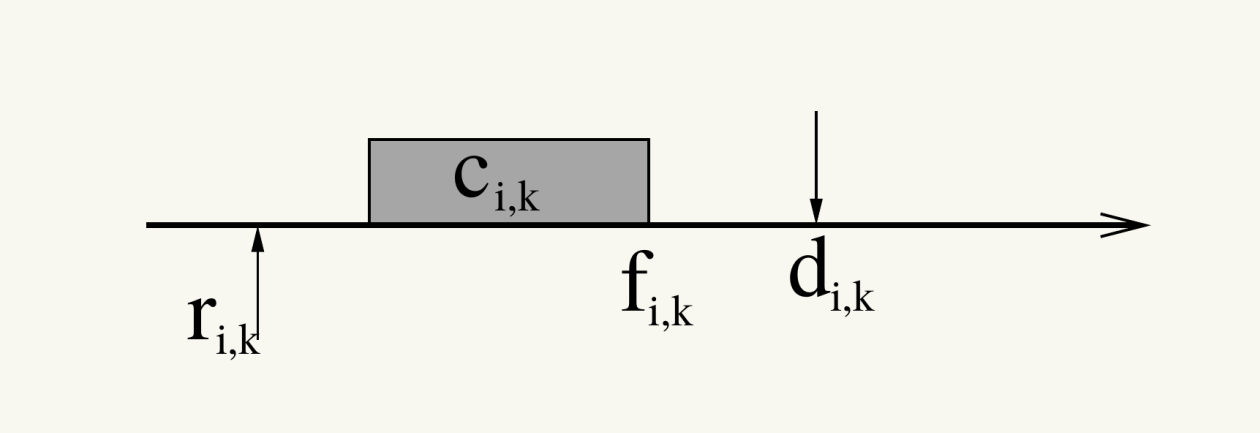
\includegraphics[width= .65\textwidth]{image01}
\end{figure}

Formally:
A job is an abstraction used to associate deadlines (temporal constraints) to activities
\begin{itemize}
\item $r_{i,k}$ time when job $J_{i,k}$ is activated (by an external event, a timer, an explicit activation, etc..)
\item $c_{i,k}$ computation time needed by job $J_{i,k}$ to complete
\item $d_{i,k}$ absolute time instant by which job $J_{i,k}$ must complete 

job $J_{i,k}$ respects its deadline if $f_{i,k} \le d_{i,k}$
\item \side{Response time} of job $J_{i,k}$
\[\rho_{i,k} = f_{i,k} - r_{i,k}\]
\end{itemize}

\subsection{Periodic Tasks}
A \side{Periodic Task} is uniquely represented by a tuple of three values in the form:
\[\tau_i = (C_i, D_i, T_i)\]
and it represents a stream of jobs $J_{i,k}$ with:
\begin{align*}
r_{i,k+1} &= r_{i,k} + T_i\\
d_{i,k} &= r_{i,k}  + D_i\\
C_i &= \max_{k}\{c_{i,k}\}
\end{align*}
where
\begin{itemize}
\item{\makebox[0.5cm]{$T_i$\hfill} is the task }\side{period}
\item{\makebox[0.5cm]{$D_i$\hfill} is the task }\side{relative deadline}
\item{\makebox[0.5cm]{$C_i$\hfill} is the task }\side{worst-case execution time (WCET)}
\item{\makebox[0.5cm]{$R_i$\hfill} is the task }\side{worst-case response time (WCRT)} defined as
\[R_i = \max_k\{\rho_{i,k}\} = \max_k\{f_{i,k} - r_{i,k}\}\]
\end{itemize}
For the task to be correctly scheduled, it must hold that:
\[R_i \le D_i\]

A periodic task has a regular structure (called \side{cycle}), in the sense that:
\begin{enumerate}
\item it is activated periodically with a period of $T_i$
\item it executes a computation
\item when the computation terminates, it suspends waiting for the next period
\end{enumerate}

Hence, its fundamental implementation can be represented as:

\begin{lstlisting}[language=C++]
void *PeriodicTask(void *arg)
{
	<initialization>;
	<start periodic timer, period = T>;
	while (condition)
	{
		<read sensors>;
		<update outputs>;
		<update state variables>;
		<wait next activation>;
	}
}
\end{lstlisting}

Tasks are graphically represented by using a \side{scheduling diagram}. For instance, figure \ref{fig:perta} shows a schedule of a periodic task 

\begin{gather*}
\tau_1 = (3,6,8)\\
WCET_1 = 3\quad D_1 = 6\quad T_1 = 8
\end{gather*}

\begin{figure}[!h]
\centering
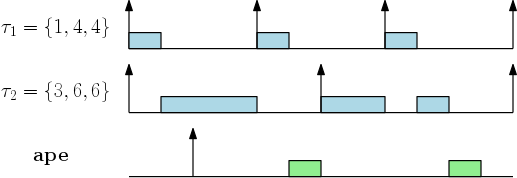
\includegraphics[width=.8\textwidth]{image02}
\caption{Periodic task graphical representation}
\label{fig:perta}
\end{figure}

Notice that, while job $J_{1,1}$ and $J_{1,3}$ execute for 3 units of time (WCET), job $J_{1,2}$ executes for only 2 units of time.

\subsection{Aperiodic Tasks}
\side{Aperiodic Task}s are not characterised by periodic arrivals, meaning that
\begin{itemize}
\item A minimum interarrival time between activations does not exist
\item Sometimes, aperiodic tasks do not have a particular structure
\end{itemize}
However, aperiodic tasks are of fundamental importance given that they model:
\begin{enumerate}
\item Tasks responding to events that occur rarely (e.g. a mode change)
\item Tasks responding to events with irregular structure (e.g. bursts of packets from the network, ...)
\end{enumerate}

A possible pattern for an aperiodic task $\tau_1$ is proposed in figure \ref{fig:aperta}

\begin{figure}[!h]
\centering
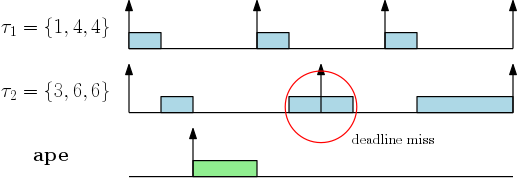
\includegraphics[width=.8\textwidth]{image03}
\caption{Aperiodic task graphical representation}
\label{fig:aperta}
\end{figure}
notive that arrivals might be bursty, and there is not a minimum time between them

\subsection{Sporadic Tasks}
\side{Sporadic Task}s are aperiodic tasks characterised by a minimum interarrival time between jobs. In this sense, they are similar to periodic tasks, but while a periodic task is activated by a periodic timer, a sporadic task is activated by an \side{external event} (e.g. the arrival of a packet from the network)

Hence, its fundamental implementation can be represented as:
\begin{lstlisting}[language=C++]
void *SporadicTask(void *arg)
{
	<initialization>;
	while (condition)
	{
		<computation>;
		<wait events>;
	}
}
\end{lstlisting}

Given its similarity with periodic task, a sporadic task can be represented by a tuple of three values
\[\tau_i = (C_i, D_i, T_i)\]
and it represents a stream of jobs $J_{i,k}$ with 
\begin{align*}
r_{i,k+1} &\ge r_{i,k} + T_i\\
d_{i,k} &= r_{i,k} + D_i\\
C_{i} &= \max_k \{c_{i,k}\}
\end{align*}
where
\begin{itemize}
\item{\makebox[0.5cm]{$T_i$\hfill} is the task }\side{minimumm interarrival time (MIT)}
\item{\makebox[0.5cm]{$D_i$\hfill} is the task relative deadline}
\item{\makebox[0.5cm]{$C_i$\hfill} is the task worst-case execution time (WCET)}
\end{itemize}
The task is correctly scheduled if $R_i \le D_i$

Since sporadic task can be represented by a mathematical model, they can be graphically displayed. Hence, figure \ref{fig:sporata} shows a possible schedule of a sporadic task $\tau_1 = (2,5,9)$.

\begin{figure}[!h]
\centering
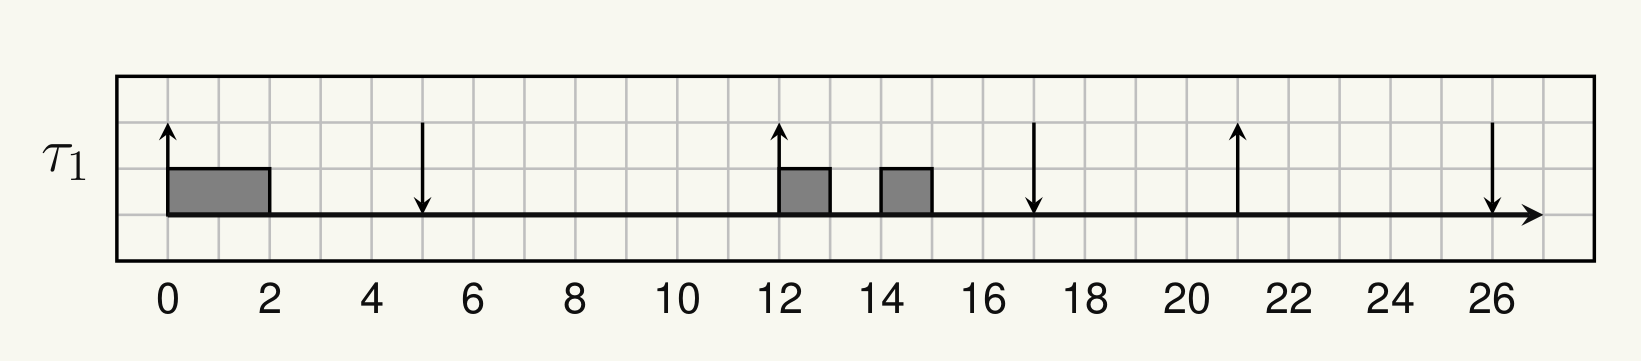
\includegraphics[width=.8\textwidth]{image04}
\caption{Sporadic task graphical representation}
\label{fig:sporata}
\end{figure}

Notice that
\begin{align*}
r_{1,2} &= 12 > r_{1,1} + T_1 = 9\\
r_{1,3} &= 21 = r_{1,2} + T_1 = 21
\end{align*}

\section{Task Criticality}
A deadline is said to be \side{hard} if  deadline miss causes a critical failure in the system, whereas a task is said to be a \side{hard real-time task} if all its deadlines are hard, which means that all the deadlines must be guaranteed before starting the task, i.e.
\[\forall j, \rho_{i,j} \le D_i \qquad\Rightarrow\qquad R_i \le D_i\]

Example:

The controller of a mobile robot, must detect obstacles and react within a time dependent on the robot speed, otherwise the robot will crash into the obstacles

A deadline is said to be \side{soft} if a deadlien miss causes a degradation in the \side{Quality of Service (QoS)}, but is not a catastrophuc event, whereas a task is said to be a \side{soft real-time task} if it has soft deadlines.

In other terms, some deadlines can be missed without compromising the correctess of the system, but the number of missed deadlines must be kept under control, because the \emph{quality} of the results depend on the number of missed deadlines.

Unline the hard real-time task, soft real-time tasks can be difficult to characterize, particularly:
\begin{itemize}
\item What's the tradeoff between ''non compromising the system correctness'' and not considering missed deadlines?
\item Moreover, some way to express the QoS experienced by a soft real-time task is needed
\end{itemize}

Exmplaes of QoS definitions could be
\begin{itemize}
\item no more than X consecutive deadlines can be missed
\item no more that X deadlines in an interval of time $T$ can be missed
\item the \side{deadline miss probability} must be less than a specified value, i.e.
\[P\{f_{i,j} > d_{i,j}\} \le R_{max}\]
\item the \side{deadline miss ratio} must be less than a specified value, i.e.
\[\cfrac{\text{number of missed deadlines}}{\text{total number of deadlines}} \le R_{max}\]
\item the maximum \side{tardiness} must be less than a specified value, i.e.
\[\cfrac{R_i}{D_i} < L\]
\item ...
\end{itemize}

A common example of implementation of a soft real-time task are the Audio and Video players. Particularly, assuming a framerate of 25 fps, which imply a frame period of 40 ms, if a frame is played a little bit too late, the user might even be unable to notice any degration in the QoS, however, \side{skipped frames} can be disturbing.

In fact missing a lot of frames by 5 ms can be better than missing only a few frames by 40 ms.

Another common example, can be found in some robotic systems where some actuations can be delayed with little consequences on the control quality.

In any case, soft real-time constraints does not mean no guarantee on dealines, given that tasks can have variable execution times between different jobs.\\
These execution times might depend on different factors:
\begin{itemize}
\item Input data
\item HW issues (cache effects, pipeline stalls, ...)
\item The internal state of the task
\item ...
\end{itemize}






















%\chapter{Real-Time scheduling and analysis}
In the previous chapter the reader was introduced to some fundamental notions and concepts that will be extensively used throughout the course.

Since, in this chapter, we will focus on the scheduling of real-time tasks and the analysis of each scheduling policy, it is worth mentioning some basic definitions:
\begin{itemize}
\item{\makebox[2cm]{Algorithm\hfill}logical procedure used to solve a problem}
\item{\makebox[2cm]{Program\hfill}formal description of an algorithm, using a programming language}
\item{\makebox[2cm]{Process\hfill}Instance of a program (program in execution)}
\begin{itemize}
\item Program: \side{static entity}
\item Process: \side{dynamic entity}
\end{itemize}
\item the term task is used to indicate a schedulable entity (either a process or a thread), in particular;
\begin{itemize}
\item A thread reresents a flow of execution (it executes with shared resources, multi thread within the same process)
\item A process represents a flow of execution + private resources (it executes with its own resources), such as address space, file table, etc...
\end{itemize}
\end{itemize}

Tasks do not run on bare hardware, but then how can multiple tasks execute on one single CPU?
The \side{OS kernel} is a piece of the operating system that takes care of multi-programming and somehow it is able to create the illusion that each CPU/processor has its own space, whereas in fact it is sharing the same resources with other processes.

In the end the kernel provides the mechanism that enable multiple tasks to execute in parallel; in a sense tasks have the illusion of executing concurrently on a dedicated CPU per task.

On this regard, with the term concurrency we refer to the simultaneous execution of multiple threads/processes in the same PC. 
\side{Concurrency} is implemented by \side{multiplexing} tasks on the same CPU. Tasks are alternated on a real CPU and the \side{task scheduler} decides which task executes at a given instant in time. In other terms, in order to implement the concurrency mechanism it is necessary to introduce this new component (i.e. the task scheduler), since it makes sure that the time of your pc is shared between the different processes or tasks that compete for the resources at that time.

Tasks are associated to temporal constraints (aka deadlines), hence the scheduler must allocate the CPU to tasks so that their deadlines are respected.

\section{Real-Time Scheduling}

One of the key components of an OS and a OS kernel is the scheduler.
A scheduler generates a schedule from a set of tasks. From a mathematical perspective it is a function:

first consider UP systems (given that it has a simpler definition).
A schedule $\sigma(t)$ is a function mapping (every point in) time $t$ into an executing task
\[\sigma : t\,\to\, \mathcal{T} \cup \tau_{idle}\]
where $\mathcal{T}$ os the \side{taskset} and $\tau_{idle}$ is the \side{idle task}.

At the end of the day what the processor/OS kernel does is to implement a function like the scheduler. Clearly, if you have more that one processor, the function under consideration is multivalued, because at every point in time it decide the allocation of the different processors to different tasks.\\
For an SMP system (i.e. $m$ CPUs), $\sigma(t)$ can be extended to map $t$ in vectors $\tau \in (\mathcal{T}\cup \tau_{idle})^m$.

Therefore, formally, the scheduler implements $\sigma(t)$ and as a consequence the scheduler is responsible for selecting the task to execute at time $t$. However, a function is a \side{denotational} way of describing an algorithm, i.e. we specify mathematically what the function is. The \side{operational} way of describing an algorithm on the other hand, is a squence of steps to be taken in order to implement the function.
 
Hence, from an operational/algorithmic point of view:
\begin{itemize}
\item \side{Scheduling algorithm} is an algorithm used to select for each time instant $t$ a task to be executed on a CPU among the ready task
\item Given a task set $\mathcal{T}$, a scheduling algorithm $\mathcal{A}$ generates the schedule $\sigma_{\mathcal{A}}(t)$
\end{itemize} 

In the frame of reference of real-time systems we are interested in finding conditions on the scheduling choice that allow us to meet all the deadlines. Hence, a task set is schedulable by an algorithm $\mathcal{A}$, if by applying that scheduling algorithm, $\sigma_{A}$ does not contain missed deadlines. 

On this note, the \side{Schedulability test} is a way to decide if, given a task set $\mathcal{T}$ and an algorithm $\mathcal{A}$, that task set is going to be schedulable.

The key point here is that given the fact that by making a proper choice of scheduling algorithm, one can obtain a schedulable task set, how can I find a way to schedule the activities so that all the deadlines are met? And this is the problem of real time scheduling.

\section{Cyclic Executive Scheduling}
One way to find a solution of the schedulability problem is to consider a task set of fixed tasks (i.e. you will always have those tasks activated in the very same way).
This is the case of legacy applications and where reliability is fundamental, e.g. military and avionics systems (Air traffic control, Space Shuttle, Boeing 777).

In this scenario, one can obtain a paper and pencil solution, i.e. trying to decide how to schedule things in such a way that the task set is schedulable and stick to that solution.

Of course, there is a more systematic way of solving such problem and such process is called \side{Cyclic Executive Scheduling}.\\
The Cyclic Executive Scheduling (aka \side{timelice scheduling} or \side{cyclic scheduling}) is a scheduling algorithm with very low overhead (in the sense that scheduling decisions are taken-offline) and with a very simple and well tested idea, that was originally used in avionic systems to schedule periodic tasks.

\subsection{The Idea}
Cyclic Executive Scheduling is a
\begin{itemize} 
\item \side{static scheduling algorithm} (i.e. it is decided offline and it is always applied repeatedly in the same way). 

As a consequence, all scheduling decision are taken upfront; it is not something that defers decision to the runtime. 
\item Jobs are assumed not to be preemptable, i.e. a scheduled job executes until termination, it retains control of the CPU for the entire computation time.
\end{itemize}
The procedure to follow in order to apply this scheduling algorithm is:
\begin{enumerate}
\item Split the time axis into slots, each of which is statically allocated to the tasks (\side{scheduling table}).
\item Since we are dealing with periodic tasks, the same sequence of tasks will repeat periodically, hence once the scheduling table is completed, it starts from the beginning and repeats the same sequence over and over again.
\end{enumerate}

A periodic timer activates execution (\side{allocation of a slot}).

In summary three components are needed to uniquely define this scheduling algorithm:
\begin{enumerate}
\item \side{Major Cycle}: least common multiple (lcm) of all the tasks' periods (aka \side{hyperperiod})
\item \side{Minor Cycle}: greatest common divison (gcd) of all the tasks' periods (i.e. granularity at which the scheduling decisions will repeat)
\item \side{A timer}: that fires every Minor Cycle ($\Delta$)
\end{enumerate}

\subsection{Implementation}
As previously mentioned from an execution stand point this scheduling algorithm is extremely simple because every minor cycle:
\begin{enumerate}
\item A periodic timer is initialized
\item Every time the timer fires the scheduler read the scheduling table
\item The scheduler calls the approriate function(s) associated to the corresponding task(s)
\item The scheduler returns to sleep until the next minor cycle (i.e. the timer fires)
\end{enumerate}

\subsection{Advantages}
From it's radical simplicity, allows to create a total check and a certification of the code that can be shipped to a space shuttle or any other avionic application and execute theoretically forever.

An OS is much more difficult to certify, because asynchronious events can be generated and it is impossible to consider upfront every possible course of events that can happen. On the contrary, once you solved the cyclic executing scheduling problem, you have a global solution that is guaranteed to be replicated.

Furthermore, with its simple implementation there is no need for a real-time operating system, no real task exist (just function calls), and only one single stack is necessary for all the \emph{tasks} (since each task runs until completion, there will never be a situation in which the execution of the function are active at the same time).

Since it involves a \side{non-preemptable scheduling} there is no critical races (i.e. there will never be two tasks that shared a variable) and therefore there is no need to protect data (i.e. no need for semaphores, pipes, mutexes, mailboxes, etc...).

Lastly, since there is no need for an OS, all the CPU/execution time is taken by the tasks, hence It has low run-time overhead, and the \side{jitter} (delay in which the result is completed, i.e. difference between when a task start and it finishes ) can be explicitly controlled.
\subsection{Drawbacks}

However, this scheduling algorithm has some important drawbacks:
\begin{itemize}
\item it is not robust w.r.t. overloads. This type of solution assumes that all the tasks do not give back control until they are finished (until its allocated slots terminates). However, if the task execute for much more of its WCET or the allocated time slot, what happens is that the schedule gets disrupted with a subsequent domino effect.
\item It is difficult to expand the schedule (static schedule): introducing a new task requires that the whole system/schedule must be redesigned.
\item Not easy to handle aperiodic/sporadic tasks
\item All task periods must be a multiple of the minor cycle time
\item Difficult to incorporate processes with long periods (big tables)
\item Variable computation time imply that it might be necessary to split tasks into a fixed number of fixed size procedures. This requires to actively change the code into smaller parts, and, in the case of third party library/code, this is not always allowed.
\end{itemize}

\section{Fixed Priority Scheduling}

In general, we want to have more flexibility than the cyclic executive scheduling (in fact it is applied on very niche and particular situations).

What can be done therefore is utilize \side{preemptive scheduling algorithm}s, i.e. algorithm that are allowed to suspend the execution of a task and resume it later.

Therefore a task has, two states: \side{ready} and \side{executing}, and the OS is allowed to enforce a state change.

In the class of preemptive algorithm we will look at different algorithms, but the simplest is the \side{Fixed Priority Scheduling}. In this scheduling algorithm:
\begin{itemize}
\item Every task $\tau_i$, when it is created, is assigned a integer number that is encoding a fixed priority $p_i$
\item The active task with the highest priority is scheduled (POSIX convention)
\end{itemize}
Priorities are integer numbers: the higher the number, the higher the priority (In the research literature, sometimes authors use the opposite convention).

And so, the work of the scheduler at any point in time is to look at the ready queue and pick up the task with the highest priority.

Observations:
\begin{itemize}
\item The response time of the task with the highest priority depends only on its computation time, and therefore it is always less than or equal to its WCET.
\item The response time of tasks with lower priority depends on its own computation time and the \side{interference} of higher priority tasks.
\item Clearly, the scheduling priorities can change how the things behave: are we sure that choosing a different priority assignment policy we would obtain a schedulable task set? Yes.

So, we have two issues: the \side{scheduling analysis} (given a task set and the priorities, is everything schedulable) and \side{syntesis problem} (given the task set and computation time, find the assignment of priorities that guarantees schedulability).
\end{itemize}

\subsection{Priority Assignment}
Given a task set how to assign priorities?\\
Depends on the different objectives that you would like to achieve:
\begin{itemize}
\item \side{Schedulability}, i.e. find the priority assignment that makes all tasks schedulable
\item \side{Response time (optimization)}, i.e. find the priority assignment that minimise the response time of a subset of tasks
\end{itemize}
By now we consider the first objective only, hence we will investigate the \side{optimal priority assignment (Opt)}.

\subsection{Optimal Priority Assignment}

A priority assignment is an optimal priority assignment (Opt):
\begin{itemize}
\item If the task set is schedulable with another priority assignment, then it is schedulable with priority assignment Opt (i.e. the optimal priority assignment cannot do any worse that any other feasible assignment).
\item If the task set is not schedulable with Opt, then it is not schedulable by any other assignment. (If the optimal choice fails then there is no other possible solutions/other alternatives will fail as well).
\end{itemize}

Formally, given a periodic task set $\mathcal{T}$ (all tasks are activated periodically) with all tasks having relative deadline $D_i$ equal to the period $T_i$ ($\forall i, D_i = T_i$), and with all offsets equal to 0 ($\forall i, r_{i,0} = 0$):
\begin{itemize}
\item The best assignment, in this case, is the \side{Rate Monotonic (RM)} assignment
\item Shorter period imply higher priority (hence the name rate monotonic: the priority is monotonic w.r.t. the rate. The higher the frequency/rate, the shorter the period, the higher the priority).
\end{itemize}

Given a periodic task set with deadline different from periods and with all offsets equal to 0 ($\forall i, r_{i,0} = 0$)
\begin{itemize}
\item The best assignment is the \side{Deadline Monotonic (DM)} assignment
\item Shorter relative deadline imply higher priority (the shorter the relative deadline, the higher the priority).
\end{itemize}
Note that the Deadline Monotonic assignment refers to relative deadline (interval in time, fixed value) not absolute deadline (instant in time, change over time).

For sporadic tasks, the same rules are valid as for periodic tasks with offsets equal to  and by considering maximum activation rate.














%\chapter{Time Demand Analysis}
%\chapter{Shared Resources}
%\chapter{Dynamic Scheduling and real world's considerations}
%\chapter{Aperiodic Servers and temporal isolation}
%\chapter{EDF Scheduling in Linux}
%\chapter{The Kernel}
%\chapter{Timer and Clock latency}
%\chapter{Non-preemtable section latency}
%\appendix
\chapter{Markov Chains}

\clearpage
\chapter*{Bibliography}
\addcontentsline{toc}{chapter}{{Bibliography}}
\printbibliography[heading=bibempty]
\end{document}